\chapter{Background estimation}

There are three main classes of backgrounds that survive the inclusive SUSY or
\smft analysis baseline selections: backgrounds with two or more prompt leptons
in the final state (giving a real SS pair), backgrounds with at least one nonprompt lepton,
and backgrounds that actually have an OS pair with one lepton having misreconstructed charge.

The first class of backgrounds are ``rare'' (have low cross section) and are estimated from
simulation, with appropriate correction factors and uncertainties to be discussed in the next
sections. This class can be further subdivided by the physical process:

\begin{itemize}
    \item \textbf{Diboson}: \\ \WZ, \ZZ, \WH, \ZH, \Zgamma, \Wgamma, and \WpWp
    \item \textbf{Triboson}: \\ \WWW, \WWZ, \WZZ, \ZZZ, \WWgamma, and \WZgamma
    \item \textbf{Single top quark and bosons}: \\ \tgamma, \tZgamma, and \tWZ
    \item \textbf{Top quark pair and one boson}: \\ \ttW, \ttZ, \ttH, and \ttgamma
    \item \textbf{Top quark pair and two bosons}: \\ \ttWW, \ttWZ, \ttZZ, \ttWH, \ttZH, and \ttHH
    \item \textbf{Triple top quark}: \\ \ttt and \tttW
    \item \textbf{Four top quarks}: \\ \tttt
\end{itemize}

In the \smft analysis, \tttt is, of course, considered a signal instead of a background.
Contributions from the first two categories of physical processes are negligible for the
\smft analysis due to the $\Nbjets\geq 2$ requirement in the baseline selections.

The second class of background events consist of events where one of the leptons is
``nonprompt'', or more colloquially, ``fake''. That is, the fake lepton is
either a real lepton which is a decay product of a heavy flavor hadron (\PQb 
or \PQc quark), or simply a misidentified hadron. The dominant sources of fake leptons
are the large cross section processes of $\ttjets$ and $\wjets$. This class is more
tricky to only use simulation, and a data-driven method is used instead.

The last class of backgrounds consists of those with a charge-misidentified lepton, or,
more colloquially ``flips'', which essentially
converts an OS pair into a SS pair. Thus, the biggest source of this background is 
the highest cross-section OS process: Drell-Yan (DY, $\PZ/\gamma\rightarrow \ell^\pm \ell^\mp$). Similarly to
the nonprompt background, this background uses a data-driven method instead of 
relying completely on simulation.

\section{Rare SM}

The large set of physics processes listed in the previous section as rare SM processes
are estimated from simulation and are grouped into larger categories, singling out
specific processes which are important to either  the inclusive SUSY analysis
or the \smft analysis. The process categories and constitutent physics processes/simulations
are:

\begin{itemize}
    \item ``$\mathbf{\ttW}$'': \ttW
    \item ``$\mathbf{\ttZ}$'': \ttZ
    \item ``$\mathbf{\ttH}$'': \ttH
    \item ``$\mathbf{\Xgamma}$'': \Wgamma, \Zgamma, \ttgamma, and \tgamma
\end{itemize}

And for the \smft analysis, there are two additional categories:
\begin{itemize}
    \item ``\textbf{Rare}'': \ttt, \tttW, \ZZ, \WH, \ZH, \WZgamma, \WWgamma, \tZgamma, \tWZ, \WpWp, and \WZ
    \item ``$\mathbf{\ttVV}$'': \ttWW, \ttWZ, \ttZZ, \ttWH, \ttZH, and \ttHH
\end{itemize}

Or, for the inclusive SUSY analysis, there are three additional categories:
\begin{itemize}
    \item ``\textbf{Rare}'': \ttt, \tttW, \ZZ, \WH, \ZH, \WZgamma, \WWgamma, \tZgamma, \tWZ, \ttWW, \ttWZ, \ttZZ, \ttWH, \ttZH, \ttHH, and \tttt
    \item ``\textbf{WZ}'': \WZ
    \item ``\textbf{WW}'': \WpWp
\end{itemize}

A breakdown of the individual processes of the ``Rare'' category in the 
\smft analysis signal regions
is shown in Figure~\ref{fig:ftraressr}, split into multi-top quark and multi-boson
processes.

Since many of these processes have not been experimentally observed or measured,
we apply conservative normalization uncertainties based on theoretical calculations of 50\% on
Rare and \Xgamma categories for the SUSY analysis, or 30\% for other categories.

\begin{figure}[!hbtp]
    \centering
    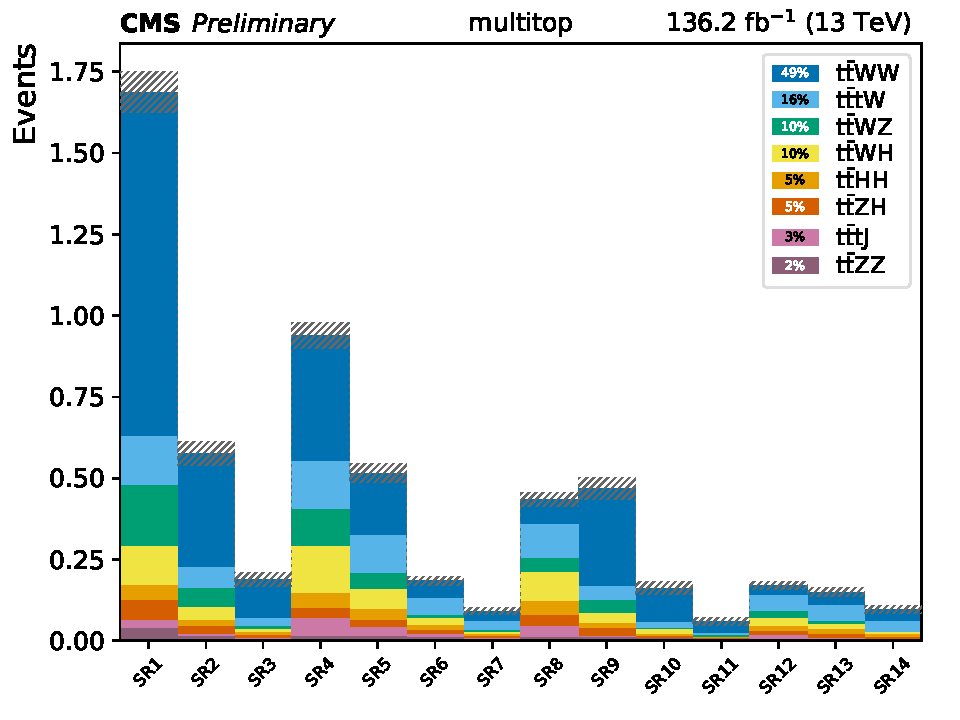
\includegraphics[width=.60\textwidth]{figs/ftan/h_multitop.pdf} \\
    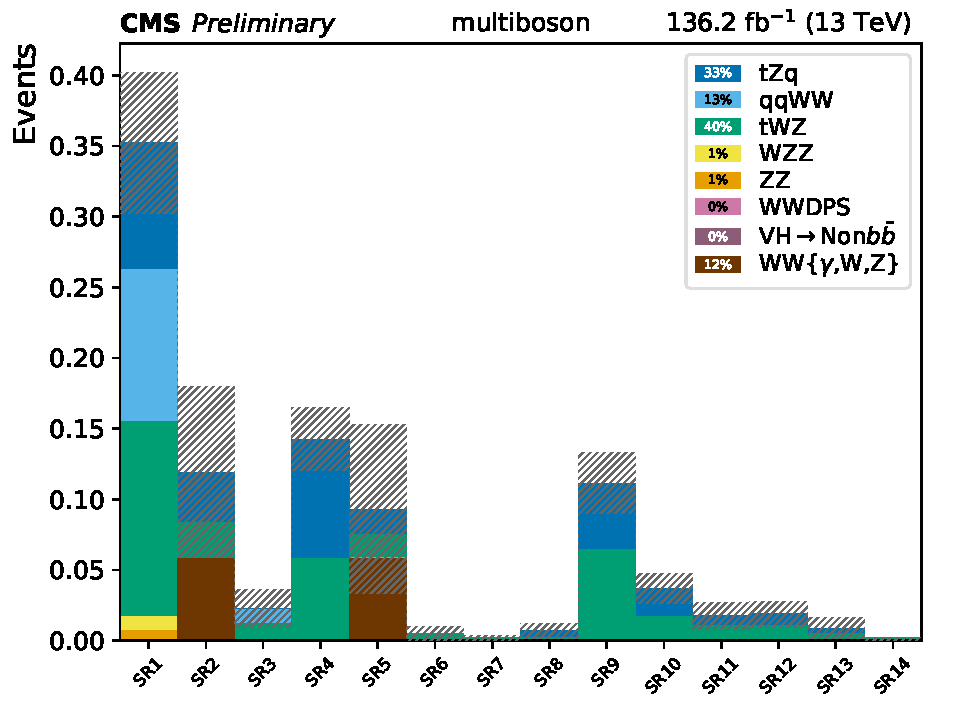
\includegraphics[width=.60\textwidth]{figs/ftan/h_multiboson.pdf}
    \caption{ Relative composition of multi-top (top) and multi-boson (bottom) rare backgrounds in the signal regions for all MC.}
    \label{fig:ftraressr}
\end{figure}

For the \smft analysis,
we apply uncertainties of 20\%, 11\%, and 11\% for Rare, \Xgamma, and \ttVV categories,
respectively, and 40\% for the \ttW and \ttZ categories. Also in the \smft analysis,
the \ttH category is assigned an uncertainty of 25\% to reflect the CMS \ttH 
measurement~\cite{CMS:Sirunyan2018hoz} which obtained a signal strength $\mu_{\ttH}$, defined
as the ratio between the measured $\ttH$ cross section and its SM expectation,
of $1.26^{+0.31}_{-0.26}$.

\FloatBarrier

\section{Nonprompt leptons}
\mytodo{todo}

\section{Charge misidentification}

The charge misidentification/flip background results from events that have
isolated OS leptons where the charge of one of the leptons is
misidentified due to mismeasurement (typical at high \pt) or bremsstrahlung.
Muons are relatively well-measured and less susceptible to radiation due to their
mass, so charge flips of muons are neglected compared to electrons.

The charge flip background is estimated by selecting OS $ee$ or $e\mu$ events 
which pass the appropriate baseline selection depending on analysis,
and then weighting the events by the \pt and $\eta$-dependent 
probability of electron charge mismeasurement, which is calculated from simulation.

The two-dimensional probability maps, shown for each of the three years of data collection 
in Fig.~\ref{fig:fliprate}, are obtained from a combination of
\ttbar and DY simulation. The probabilities
are then validated using a control sample in data of
SS $\PZ\rightarrow e^\pm e^\pm$ baseline events, 
instead using a $\ptmiss<50\GeV$ requirement to be
orthogonal to the signal regions. 
The level of disagreement in this control region
is used to assess the associated systematic uncertainty and to derive a
correction to the MC-based rate estimation.  In the 2016 data sample, we find good
agreement between prediction and data in the control region.
However, in the 2017 and 2018 data samples, the MC-based flip rate
is significantly lower than for
2016 due to the upgraded pixel detector (which added an extra inner pixel layer),
so the obsered number of events in the
SS $\PZ\rightarrow e^\pm e^\pm$ region is found to be nearly 40\% higher than the
predicted number of events. Consequently, the 2017 and 2018 charge
flip predictions are scaled up by approximately 40\%, as seen in
Figure~\ref{fig:flipclosure}. These year-by-year correction factors are summarized in
Table~\ref{tab:flipscaling}. Since we do not observe significant trends
in the lepton kinematics, we do not consider \pt and $\eta$-binned
corrections on top of the tabulated flat correction factors. 
In addition to the statistical uncertainties, we apply a 20\%
systematic uncertainty on this background prediction for all years. In MC, the
flip rate for muons is found to be an order of magnitude smaller than for
electrons and is therefore neglected, as it would in any case be covered by
the systematic uncertainty of 20\% on this background.



\begin{table}[h]
  \begin{center}
    \small
    \begin{tabular}{c|c}
      \hline
      year & observation/prediction \\
      \hline
        2016 & 1.01  \\
        2017 & 1.44  \\
        2018 & 1.41  \\
      \hline
    \end{tabular}
    \caption{ Ratio of observed flip rate in data to the flip rate prediction from simulation.
     These are the multiplicative correction to the MC-based charge flip probabilities. }
    \label{tab:flipscaling}
  \end{center}
\end{table}

\begin{figure}[!hbtp]
\centering
\centering
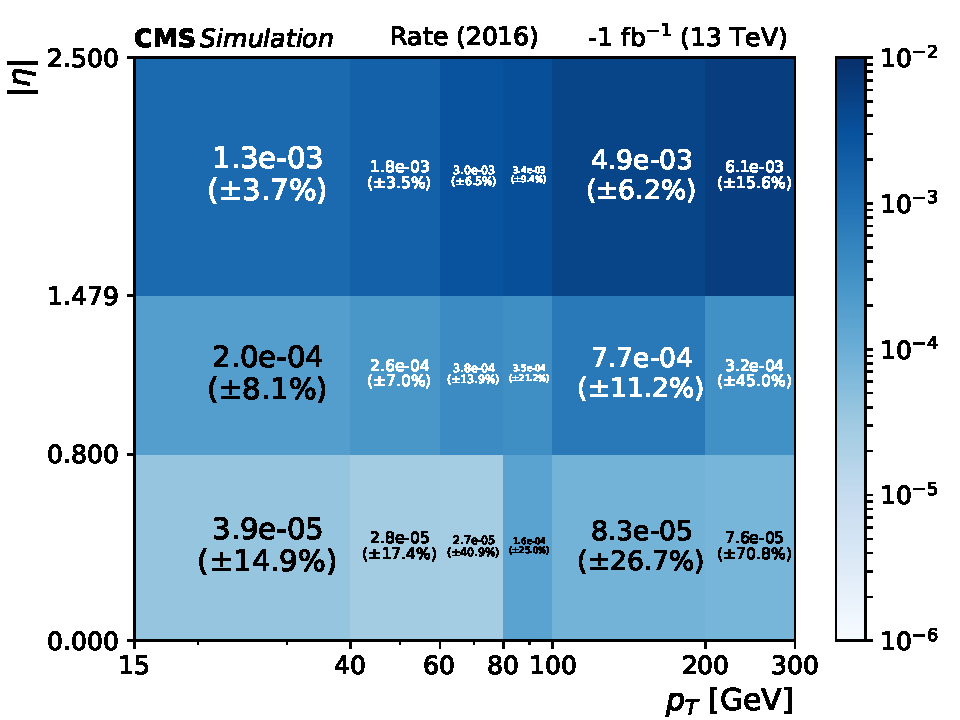
\includegraphics[width=.48\textwidth]{figs/ftan/flips/y2016/fliprate.pdf}
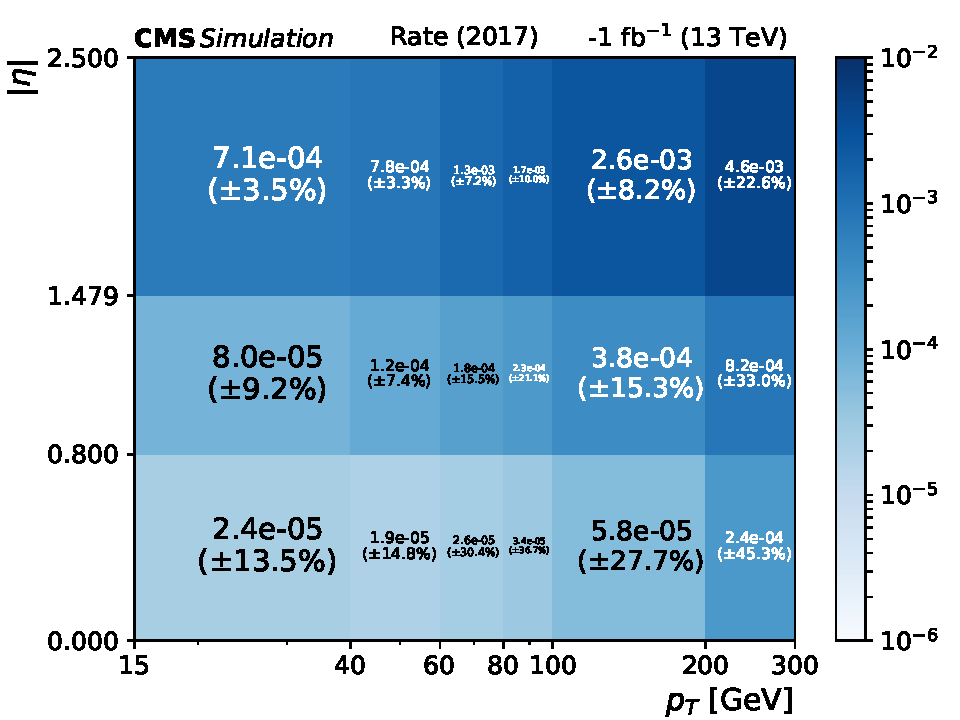
\includegraphics[width=.48\textwidth]{figs/ftan/flips/y2017/fliprate.pdf}
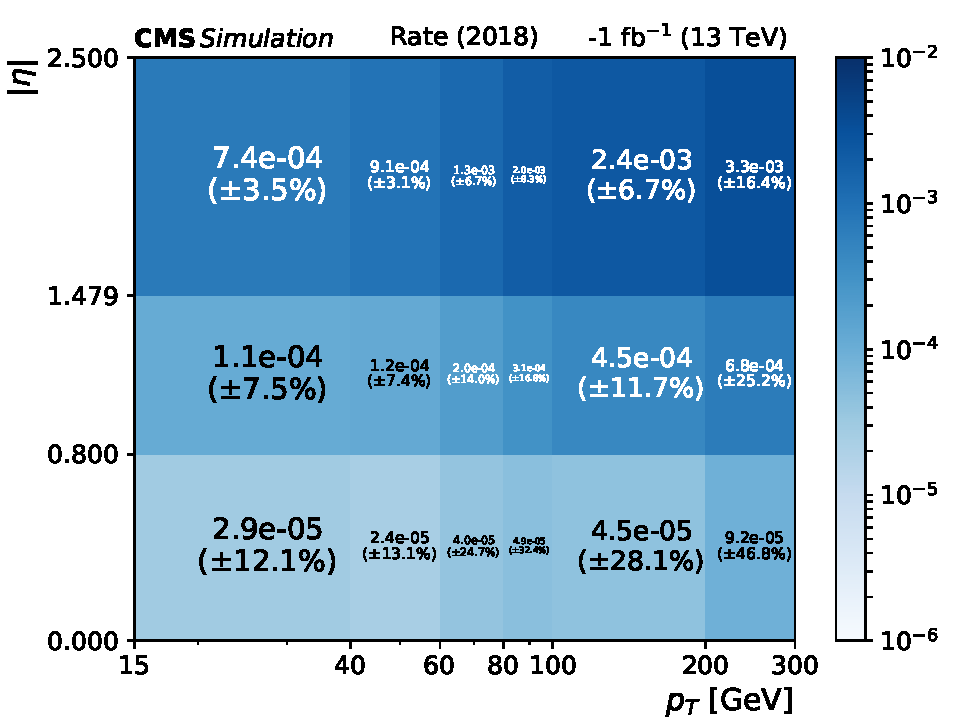
\includegraphics[width=.48\textwidth]{figs/ftan/flips/y2018/fliprate.pdf}
\caption{ Electron charge flip rate for 2016, 2017, and 2018. }
\label{fig:fliprate}
\end{figure}

\begin{figure}[!hbtp]
\centering
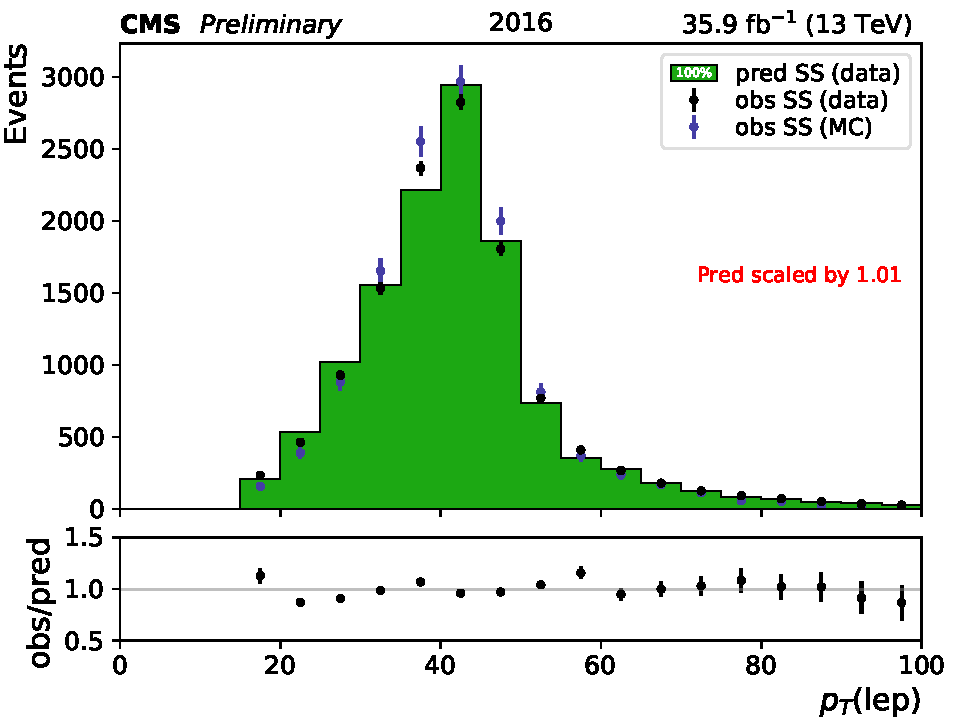
\includegraphics[width=.31\textwidth]{figs/ftan/flips/y2016/leppt.pdf}
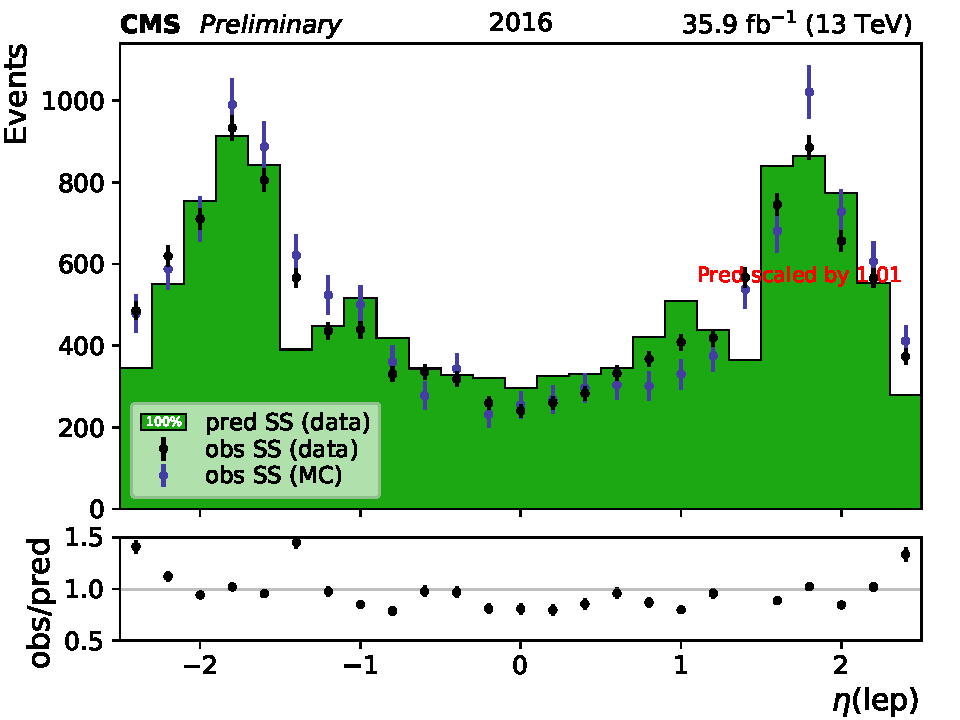
\includegraphics[width=.31\textwidth]{figs/ftan/flips/y2016/lepeta.pdf}
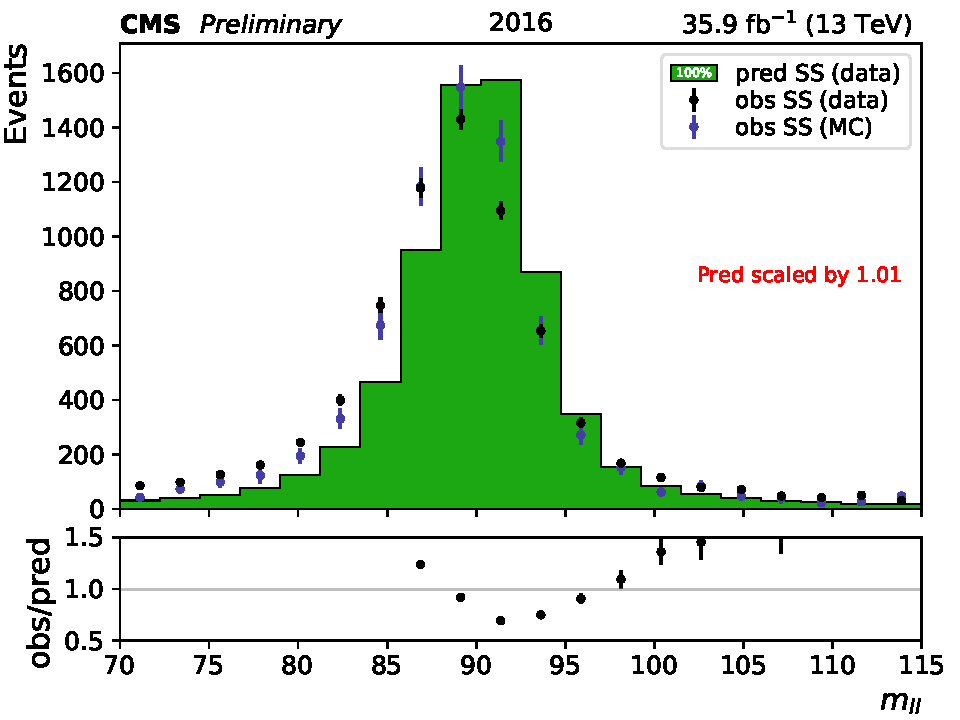
\includegraphics[width=.31\textwidth]{figs/ftan/flips/y2016/mll.pdf} \\
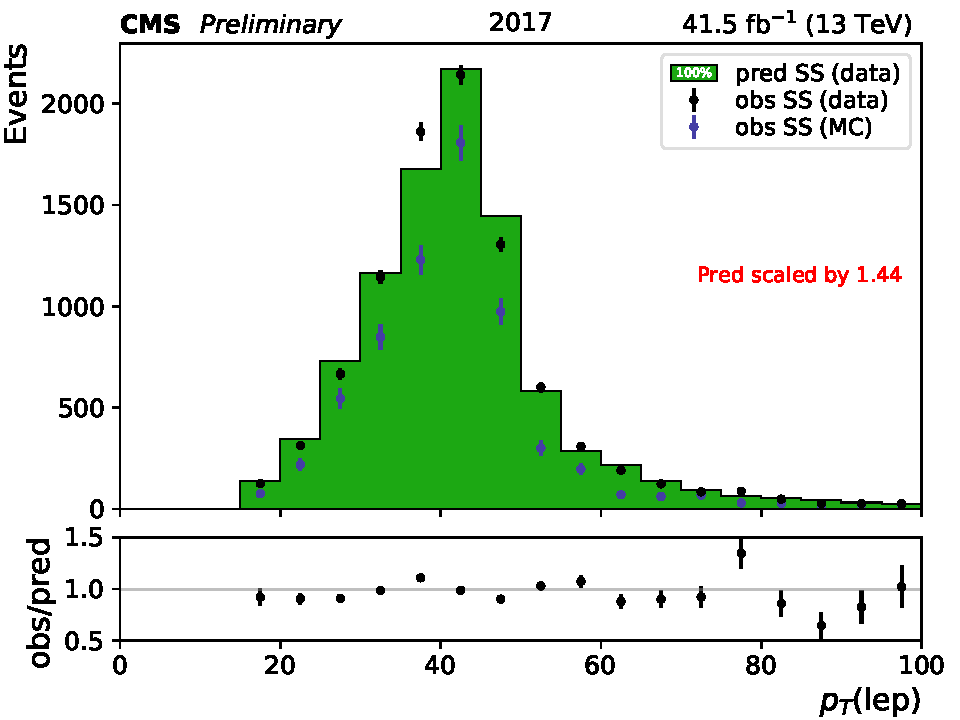
\includegraphics[width=.31\textwidth]{figs/ftan/flips/y2017/leppt.pdf}
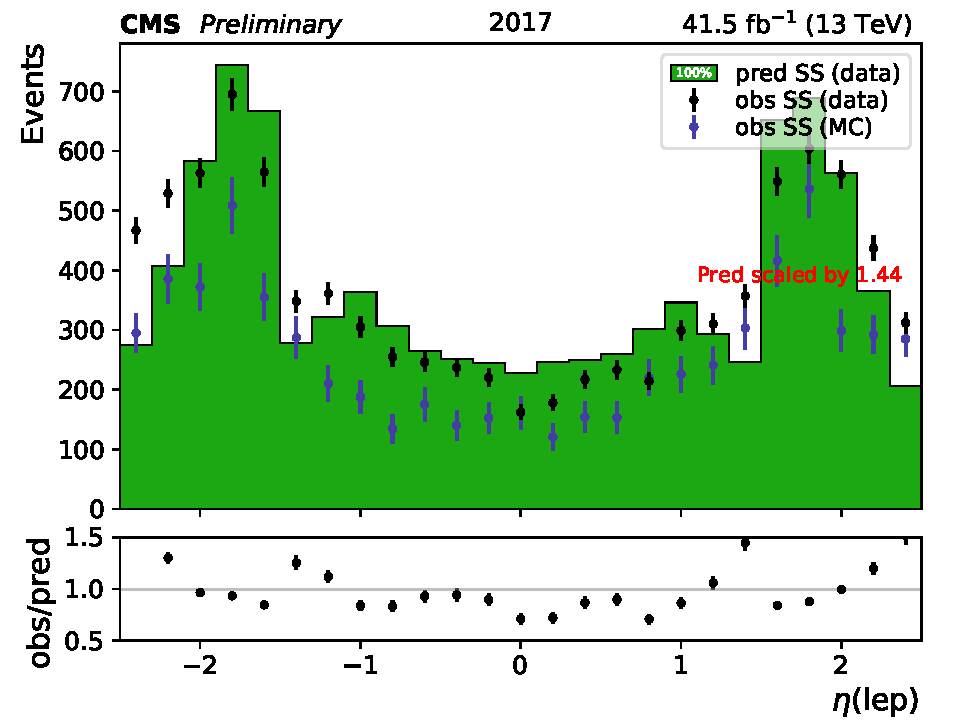
\includegraphics[width=.31\textwidth]{figs/ftan/flips/y2017/lepeta.pdf}
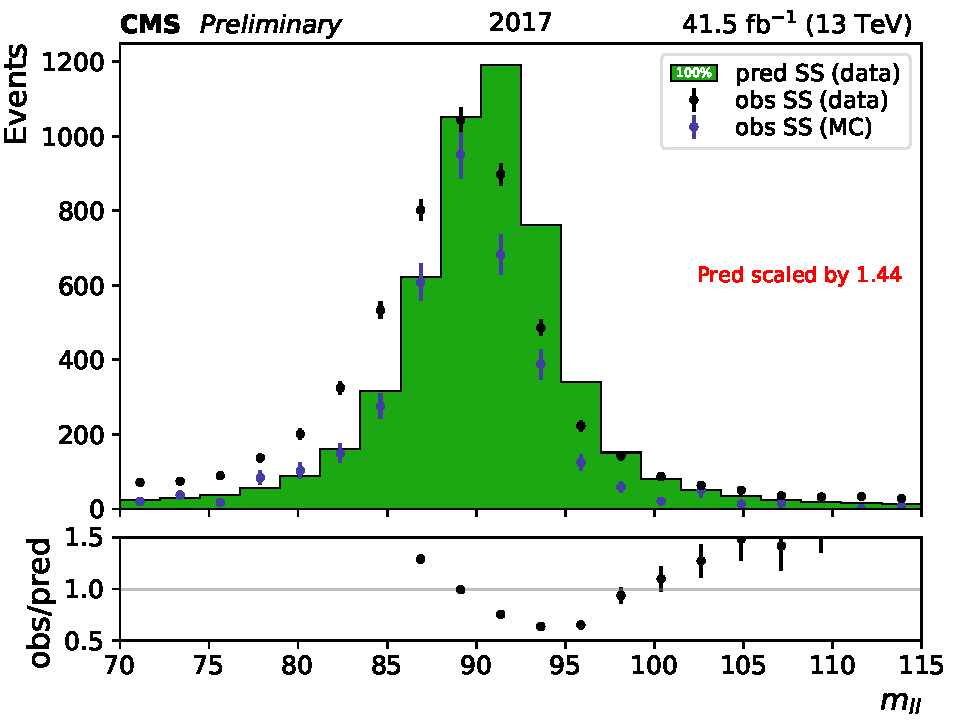
\includegraphics[width=.31\textwidth]{figs/ftan/flips/y2017/mll.pdf} \\
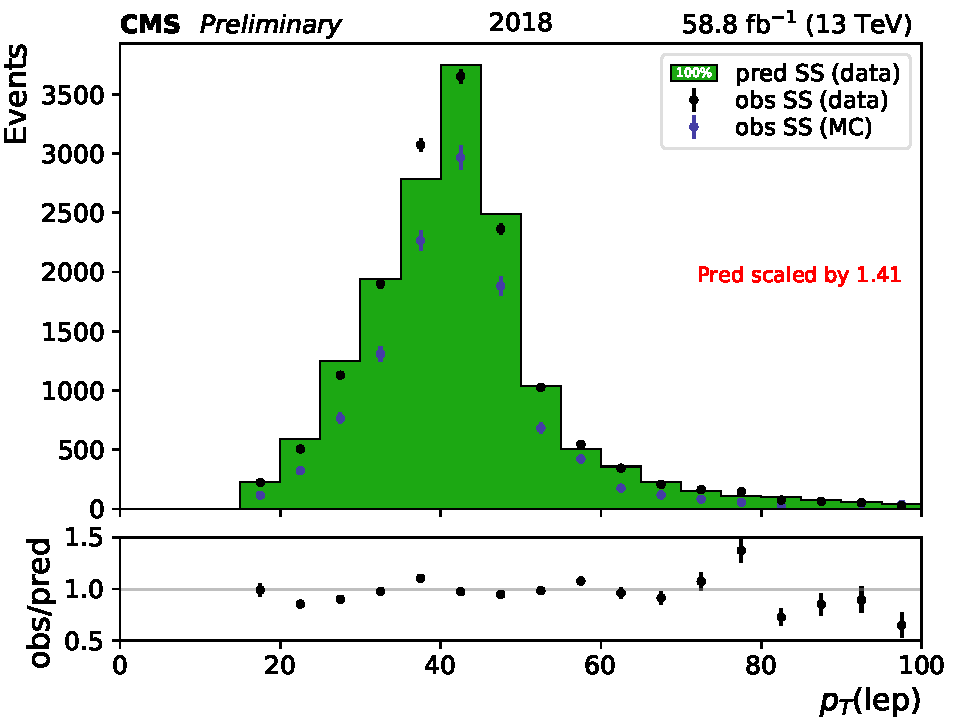
\includegraphics[width=.31\textwidth]{figs/ftan/flips/y2018/leppt.pdf}
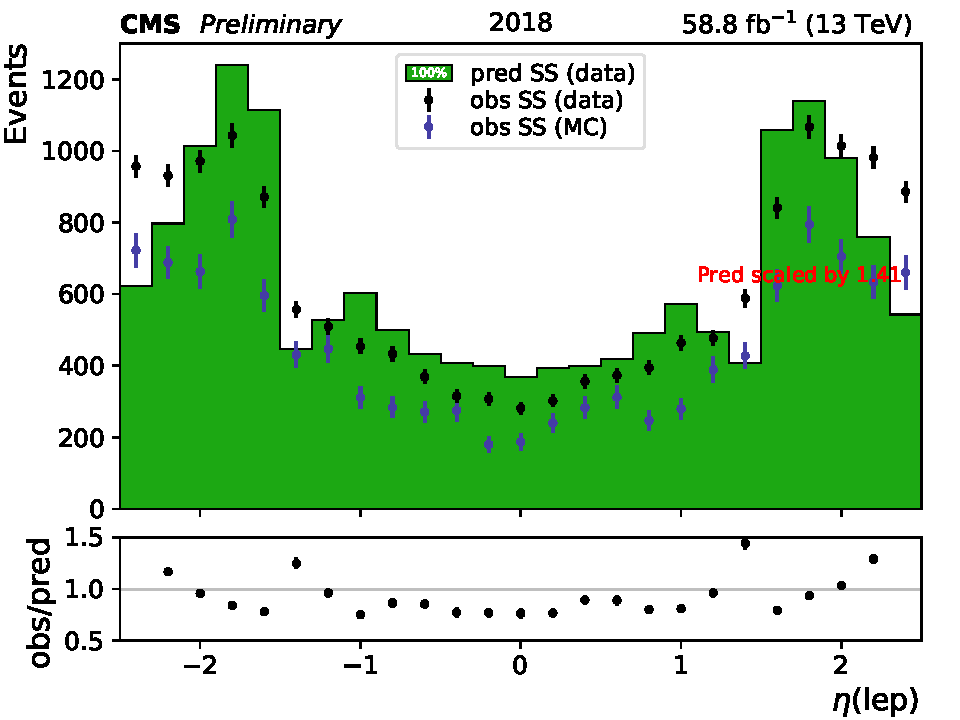
\includegraphics[width=.31\textwidth]{figs/ftan/flips/y2018/lepeta.pdf}
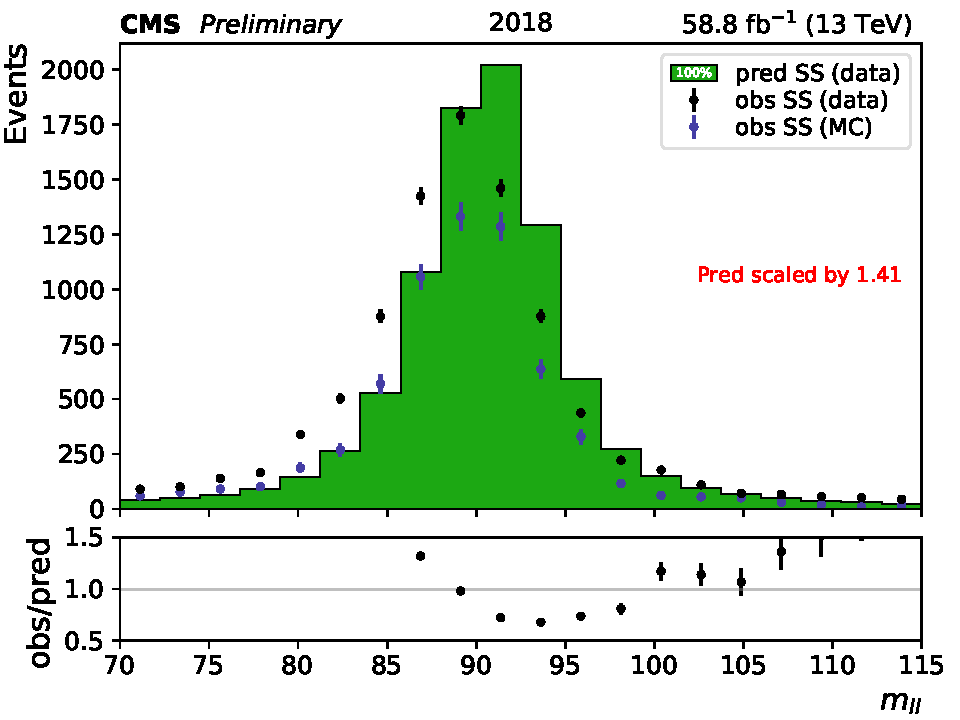
\includegraphics[width=.31\textwidth]{figs/ftan/flips/y2018/mll.pdf} \\
    \caption{  Predicted and observed lepton \pt (left) and $\eta$ (middle) and $m_{\ell\ell}$ (right) in a SS $\PZ \rightarrow e^\pm e^\pm$ peak
    for the years 2016, 2017, and 2018, from top to bottom.
The prediction is normalized to the observed data with the normalization factor inset in red.
The filled green histogram consists of predicted charge flip events (reweighted OS events),
the black points consist of observed charge flip events in data (SS), and the blue points
show the observed charge flip events in MC (SS).
}
\label{fig:flipclosure}
\end{figure}

\FloatBarrier

\section{Corrections}
\mytodo{todo}

In addition to corrections associated with JEC, \PQb-tagging, lepton scale factors,
and trigger scale factors, mentioned throughout previous sections and chapters, we
apply some dedicated corrections to simulation to bring better agreement between data
and simulation.

\mytodo{ttbb}

\mytodo{nisr}

\section{Control regions}
\mytodo{todo}

\section{Systematic uncertainties}
\mytodo{todo}

